\documentclass[dvipsnames]{article}
\usepackage{pgfplots}
\usetikzlibrary{decorations.markings}
\pgfplotsset{compat=newest}

% \def\Point{36.9}

\begin{document}

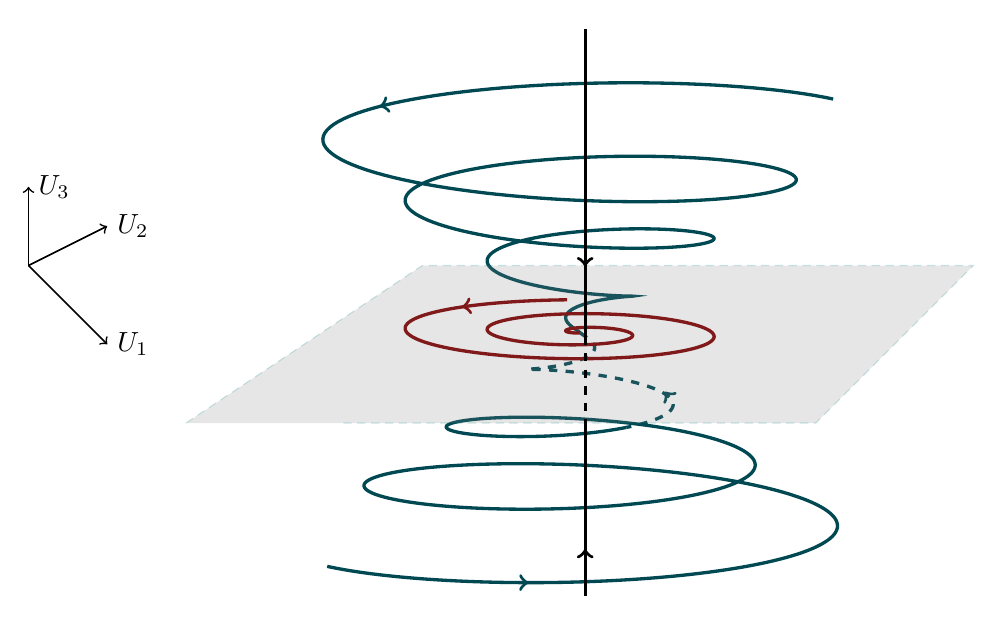
\begin{tikzpicture}
%левая
  \begin{axis}[
    view={-50}{-10}, %угол обзора
    axis lines=none,
    zmax=60,
    height=10cm,
    xtick=\empty,
    ytick=\empty,
    ztick=\empty
    ]
    \addplot3+[,ytick=\empty,yticklabel=\empty,
    mark=none,
    very thick,
    color={rgb,255:red,0; green,73; blue,83},
    domain=0:15*pi,
    postaction={decorate,
                decoration={markings,mark=at position 0.8 with {\arrow{<}}}
               },
    samples=400,
    samples y=0,
    ]
    (-{x*sin(0.15*pi*deg(x))},{x*cos(0.15*pi*deg(x)},{x});
    ]
    \addplot3+[,ytick=\empty,yticklabel=\empty,
    mark=none,
    dashed, very thick,
    color={rgb,255:red,0; green,73; blue,83},
    domain=0:-5.5*pi,
    postaction={decorate,
                decoration={markings,mark=at position 0.8 with {\arrow{<}}}
               },
    samples=400,
    samples y=0,
    ]
    (-{x*sin(-0.15*pi*deg(x))},{x*cos(0.15*pi*deg(x)},{x});
    ]

    \addplot3+[,ytick=\empty,yticklabel=\empty,
    mark=none,
    very thick,
    color={rgb,255:red,0; green,73; blue,83},
    domain=-5.5*pi:-15*pi,
    postaction={decorate,
                decoration={markings,mark=at position 0.9 with {\arrow{<}}}
               },
    samples=400,
    samples y=0,
    ]
    (-{x*sin(-0.15*pi*deg(x))},{x*cos(0.15*pi*deg(x)},{x});

  \addplot3+[,ytick=\empty,yticklabel=\empty,
    mark=none,
    very thick,
    color={rgb,255:red,128; green,0; blue,0},
    domain=0:10*pi,
    postaction={decorate,
                decoration={markings,mark=at position 0.9 with {\arrow{<}}}
               },
    samples=400,
    samples y=0,
    ]
    (-{x*sin(0.15*pi*deg(x))},{x*cos(0.15*pi*deg(x)},{0});
    ]

  \end{axis}
  \draw[teal,densely dashed][fill = gray, opacity=0.2]  (0,3) -- (3,5) -- (10,5) -- (8,3) -- (2,3);
  \draw[very thick] [->] (5.07,5) --(5.07,4.99);
  \draw[very thick] (5.07,8) --(5.07,4.1);
  \draw[very thick, dashed] (5.07,4.1) --(5.07,3);
  \draw[very thick] (5.07,3) --(5.07,0.8);
  \draw[very thick] [->] (5.07,1.39) --(5.07,1.4);
  \draw[semithick] [->] (-2,5) -- (-1,4) node[right] {$U_1$};
  \draw[semithick] [->] (-2,5) -- (-1,5.5) node[right] {$U_2$};
  \draw[semithick] [->] (-2,5) -- (-2,6) node[right] {$U_3$};
\end{tikzpicture}

\end{document}